\graphicspath{{./assets/}}
\setcounter{mtc}{10}
\chapter{8th Sprint: Deployment of the authentication/authorization platform }
\fancyhead[R]{\ungaramond\small\textbf{Chapter X. 8th Sprint: Deployment of the authentication/authorization platform }}

\minitoc
\newpage
\subsection*{Introduction}
Security is of utmost importance, especially when it comes to protecting sensitive information. Authentication and authorization platforms play a critical role in ensuring that only authorized individuals have access to valuable resources. 

In this chapter, we will explore the various components involved in securing access and their configuration and deployment. 


\subsection{Sprint backlog :}

\begin{longtable}[H]{|m{1.5cm}|m{3cm}|m{1.5cm}|m{9cm}|}
\hline
{\textbf{Epic ID}} & {\textbf{Epic}} & {\textbf{Story ID}} & {\textbf{Story}}\\
\hline
1  & Deployment of the authentication/authorization backend.  &  1.1	 & Deployment and configuration of authentication and authorization services.\\
\cline{3-4}
& & 1.2 & Configuring the forward auth middleware for secure access.  \\
\cline{3-4}
\hline
\caption{8th Sprint Backlog}
\end{longtable}
\section{Authentication and authorization}
\subsection{Conceptual overview }

Previously, traefik has been deployed and configured to serve as an ingress controller and load balancer for our platform as a service. In this chapter we discuss how an assortment of components are used in combination with traefik to provide a secure and scalable solution for authentication and authorization. 

The following diagram illustrates the layout of this architecture: 

\begin{figure}[H]\centering
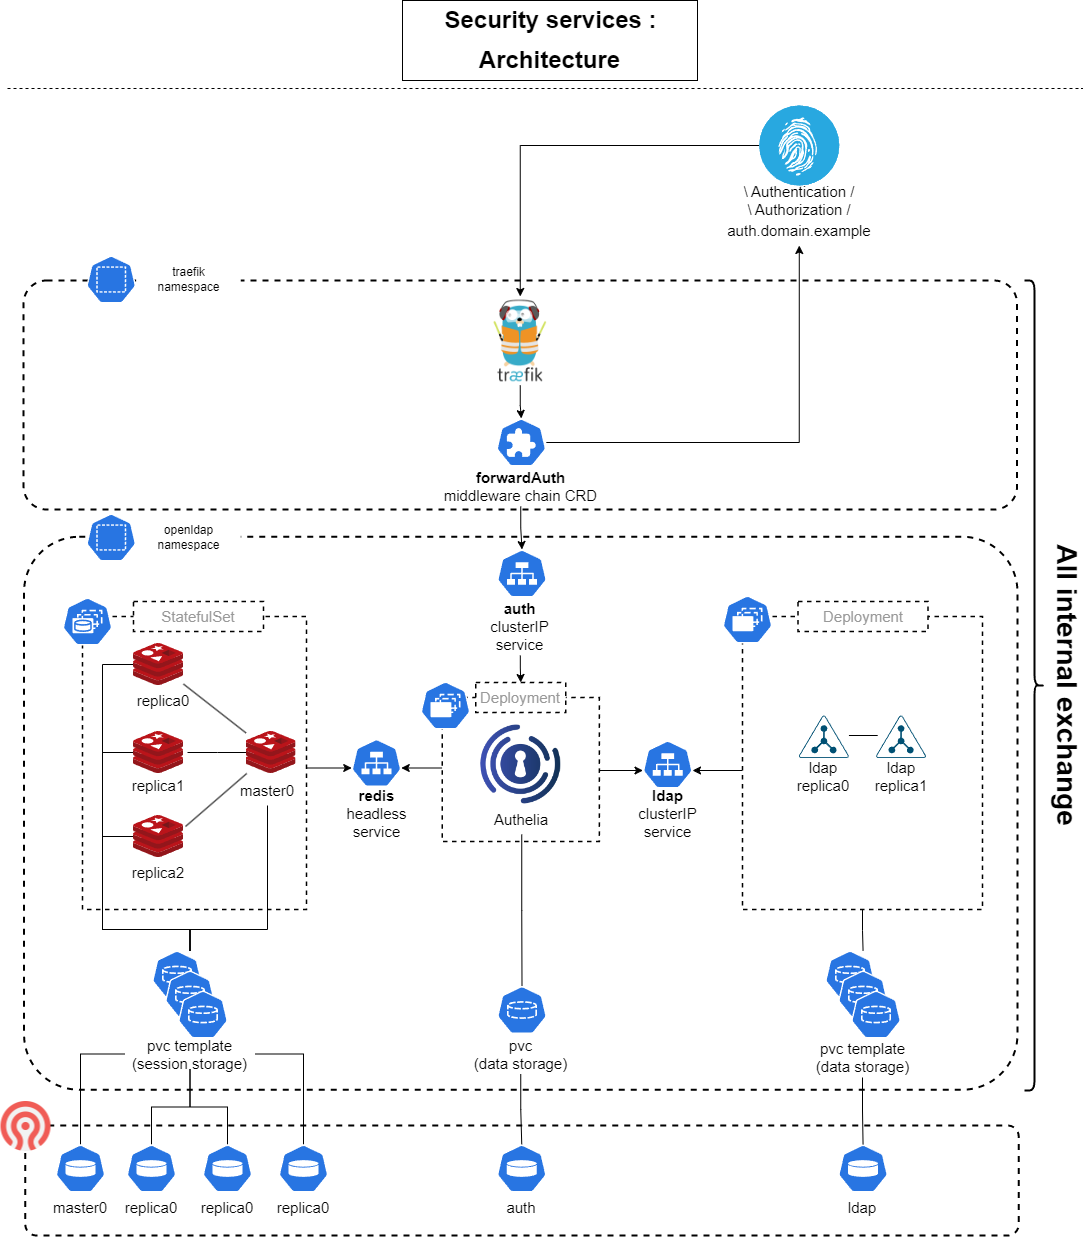
\includegraphics[width=1.0\textwidth,angle=00]{assets/f51.png}
\caption{Conceptual overview }
\label{fig:f51}
\end{figure}

\textbf{Traefik} is used as a reverse proxy and ingress controller, which allows external traffic to access the applications running inside the Kubernetes cluster. Traefik provides load balancing, SSL termination, and routing based on rules defined in its configuration. 

\textbf{Authelia} is used as a forward authentication and authorization controller, which provides an additional layer of security by enforcing authentication and authorization before requests are forwarded to the backend services. Authelia also provides Single Sign-On (SSO) functionality, allowing users to authenticate once and access multiple applications seamlessly. 

\textbf{OpenLDAP}, which stores user information and credentials for authentication and authorization purposes, is used as an LDAP server in conjunction with a web interface to facilitate management. 

Authelia authenticates users against the OpenLDAP server and authorizes access to resources based on LDAP group membership. 

\textbf{Redis} is used for session storage, which stores user session information to ensure that users remain authenticated and authorized throughout their session. 

 

\subsection{Deployment and configuration of components }

\subsubsection{openLDAP for access and user management  }

A custom openldap server is deployed for the purpose of safely and reliably accessing and managing the distributed directories that store information about users, groups, resources. 

\subsubsubsection{Deployment: }

An ansible playbook is firstly run to perform the following steps : 
\begin{itemize}[label={--}]
\item Using the “community.docker.docker\_image” library, building the custom container image of the openLDAP server as well as the web interface. 
\item Using the “community.docker.docker\_image” library, pushings the built images to the private registry. 
\item Using the “kubernetes.core.k8s” library, applying the manifests to deploy the server. 
\end{itemize}

The following is a code snippet from the manifest for deploying the openLDAP server: 

\begin{listing}[H]
\inputminted[firstline=1,lastline=10]{Yaml}{codeListing/deploy_openldap.yml}
\end{listing} 

\begin{listing}[H]
\inputminted[firstline=16,lastline=55]{Yaml}{codeListing/deploy_openldap.yml}
\end{listing} 

\begin{listing}[H]
\inputminted[firstline=56]{Yaml}{codeListing/deploy_openldap.yml}
\caption{Deploying openLDAP}
\label{lst:Deploying_openLDAP}
\end{listing} 

\subsubsubsection{Resource overview }

The web interface below is deployed and configured to provide secure remote access to the openLDAP server entries, thus allowing management operations. This is achieved using the LDAP base name of the company. Naturally, external direct access to server is prohibited. 
\begin{figure}[H]\centering
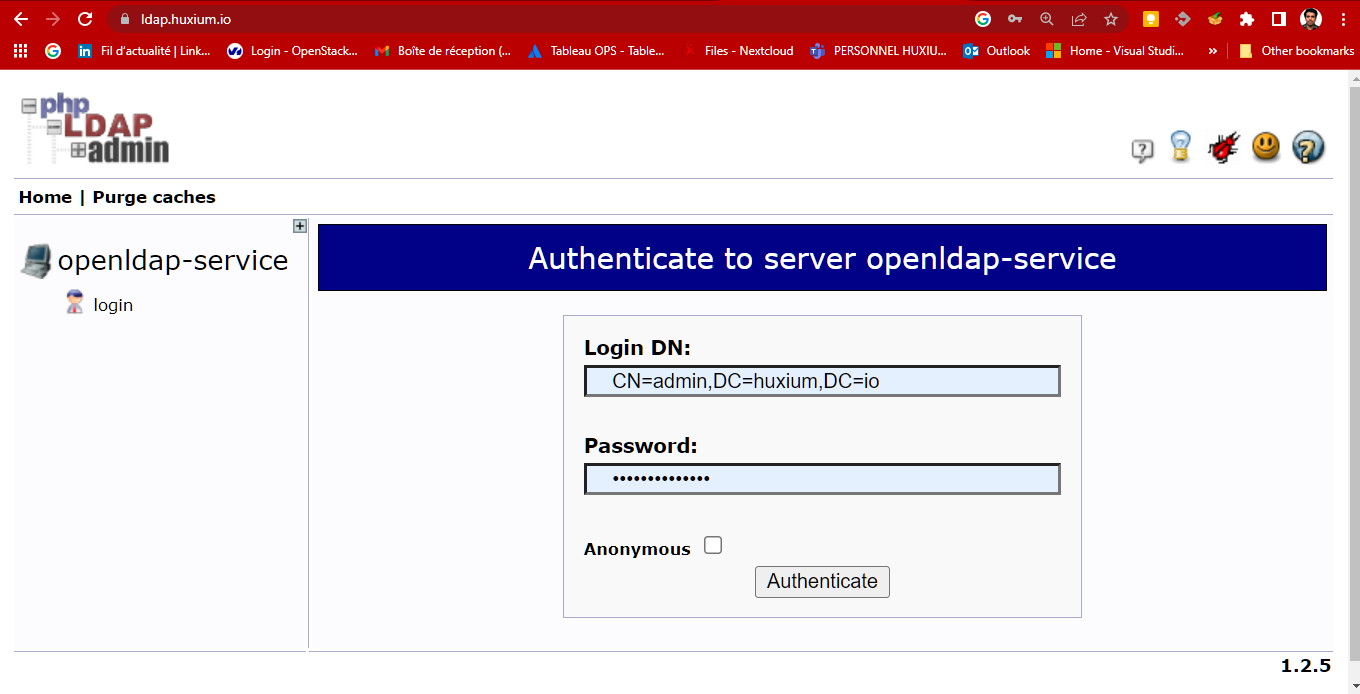
\includegraphics[width=1.0\textwidth,angle=00]{assets/f52.png}
\caption{Figure 52 }
\label{fig:f52}
\end{figure} 

\subsubsection{Redis for session storage }

Redis is used with the “auth-middleware” for session storage because Redis is an efficient and highly scalable in-memory data store that can handle high-traffic web applications. 

\subsubsubsection{Deployment:} 

When users log in, their authentication and session data are stored in a session cookie, which is used to authenticate them on subsequent requests. 

By using Redis as the session store for Authelia, it becomes possible to store these session cookies in a highly available and scalable data store that can be shared across multiple Authelia instances.  

This is important for applications that experience heavy traffic, as it ensures that user authentication data can be retrieved and verified quickly and efficiently. 

\subsubsubsection{Resource overview: }

The following is an overview of the resulting ReplicaSet for Redis: 

\begin{figure}[H]\centering
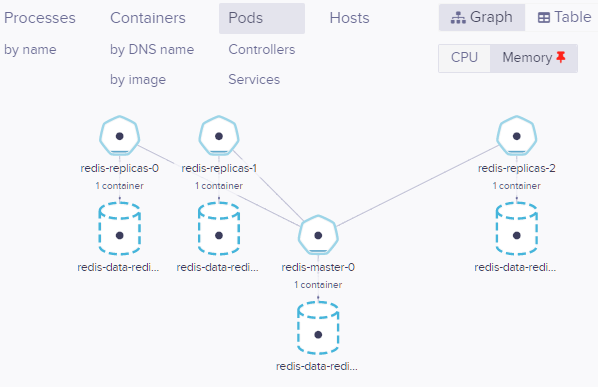
\includegraphics[width=1.0\textwidth,angle=00]{assets/f53.png}
\caption{Figure 53 }
\label{fig:f53}
\end{figure}

The ReplicaSet contains 4 pods with a persistent volume each. The pod hierarchy is as follows: 
\begin{itemize}[label={--}]
\item One master pod with the read/write privilege. 
\item Three replicas with read-only access. 
\end{itemize}
Only internal access is allowed. This is achieved using the following services: 

\begin{itemize}[label={--}]
\item redis-master.openldap.svc.cluster.local for read/write operations (port 6379) 
\item redis-replicas.openldap.svc.cluster.local for read-only operations (port 6379) 
\end{itemize}



\subsubsection{Authelia for single sign-on }

Authelia is put in place to provide a single sign-on experience and fine-grained access control for applications and services running on the cluster.  

\subsubsubsection{Deployment: }

It leverages the LDAP server to cross-check user credentials. Two backend database servers are configured. Authelia uses the HA PostgreSQL cluster to store policies and other data. It also relies on the replicated Redis cluster for user session storage. 

The following configuration is attached to the authelia containers using the configmap binding method: 

\begin{listing}[H]
    \inputminted[firstline=1,lastline=25]{Yaml}{codeListing/authelia_configmap.yml}
\end{listing}

\begin{listing}[H]
    \inputminted[firstline=26,lastline=55]{Yaml}{codeListing/authelia_configmap.yml}
\end{listing}

\begin{listing}[H]
    \inputminted[firstline=56]{Yaml}{codeListing/authelia_configmap.yml}
    \caption{Authelia configuration}
    \label{lst:Authelia configuration}
\end{listing}

\subsubsubsection{Resource overview : }

The following is an overview of the deployed resources: 
\begin{figure}[H]\centering
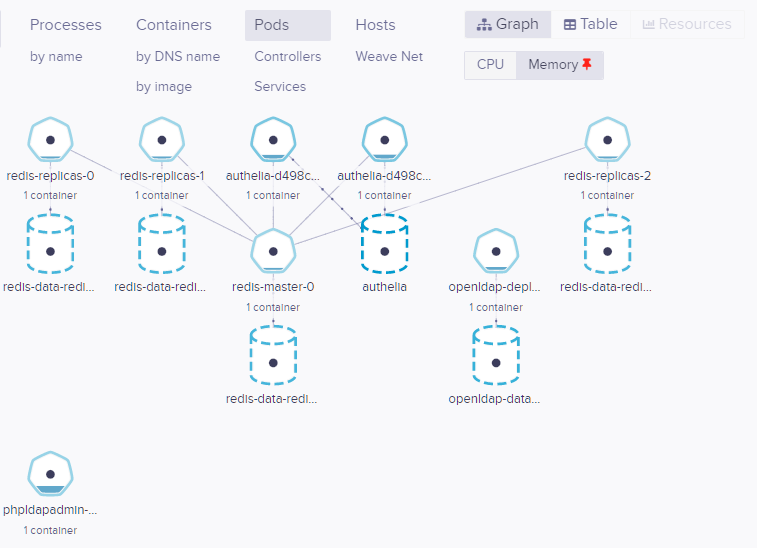
\includegraphics[width=1.0\textwidth,angle=00]{assets/f54.png}
\caption{Deployed resources}
\label{fig:f54}
\end{figure}


This diagram features the following elements: 

\begin{itemize}[label={--}]
\item A deployment of authelia configured with a horizontal pod autoscaler.  
\item The replicated Redis cluster to stora session data. 
\item The openLDAP server that houses user credentials. 
\end{itemize}

Each of these workloads has volumes attached to it in order to persist data. 

\subsection{The authentication gateway in action }

\subsubsection{Preliminary configuration }

As a first step, the “Middleware CRDs” that handle the request forwarding is configured. 

Naturally, communication between the ingress controller, Traefik, and the authentication server, Authelia, is exchanged internally in the cluster. 

\subsubsubsection{The “forward-auth” middleware }

Forward authentication with Traefik means that incoming requests to a service are first authenticated by the authentication server, Authelia, before being forwarded to the service. 

The following is the code snippet of this declaration: 

\begin{listing}[H]
    \inputminted{Yaml}{codeListing/middleware_forward_auth.yml}
    \caption{forward-auth middleware}
    \label{lst:forward-auth middleware}
\end{listing}

The “headers” middleware 

The “headers” middleware is a collection of middleware components that are used to authenticate and authorize HTTP requests based on various headers.  

\begin{listing}[H]
    \inputminted{Yaml}{codeListing/middleware_headers.yml}
    \caption{headers middleware}
    \label{lst:headers middleware}
\end{listing} 

These headers can include the Authorization header, session cookies, and other custom headers that contain authentication information. 

\subsubsection{Implementation }

\subsubsubsection{The authentication portal }

A chain of the “Middleware CRDs” declared above is leveraged in the following  ingressroute to deploy the authentication portal: 

\begin{listing}[H]
\inputminted{Yaml}{codeListing/authelia_ingressroute.yml}
\caption{authelia ingressroute}
\label{lst:authelia ingressroute}
\end{listing}

The following figure shows the authentication portal as seen by an external user: 
\begin{figure}[H]\centering
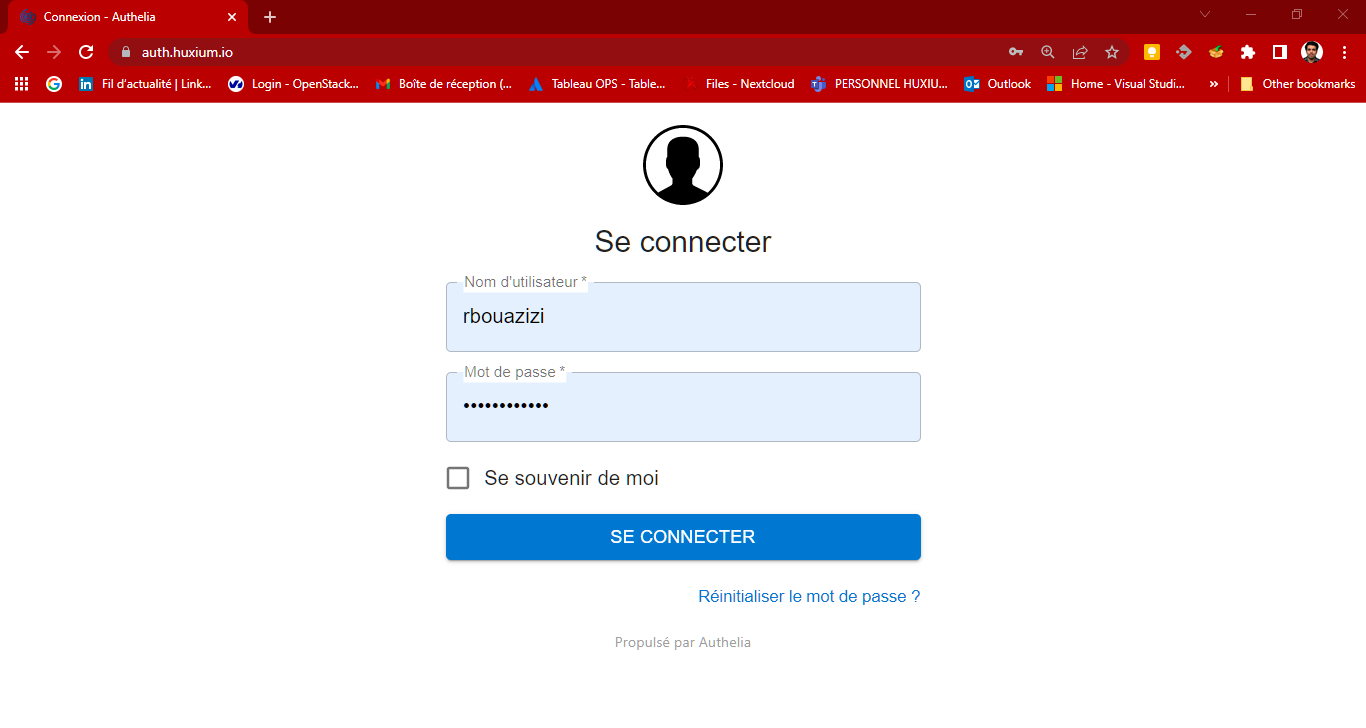
\includegraphics[width=1.0\textwidth,angle=00]{assets/f55.png}
\caption{Authentication portal}
\label{fig:f55}
\end{figure}

\subsubsubsection{How it works }

The architecture works as follows: 
\begin{itemize}[label={--}]
\item The user sends a request to access a protected resource. 
\item  Traefik receives the request and forwards it to Authelia. 
\item  Authelia authenticates the user against the OpenLDAP server and checks the user's group membership to determine whether access is authorized. 
\item  If the user is authenticated and authorized, Authelia sets up a session for the user and sends a token to Traefik. 
\item  Traefik receives the token and sets it as a cookie in the user's browser for subsequent requests. 
\item  For subsequent requests, Traefik checks the cookie for a valid token and forwards the request to the backend service if the token is valid. Otherwise, the user is redirected to the authentication page.  
\end{itemize}

\subsection*{Conclusion}

In conclusion, deploying an authentication and authorization platform on Kubernetes using Traefik, Authelia, OpenLDAP, and Redis can provide a secure and scalable solution for managing user access to resources. 

By leveraging the power of Kubernetes, we can easily manage and scale the platform, ensuring high availability and fault tolerance. 

The use of Traefik as a reverse proxy provides secure communication between the user and the platform, while Authelia and OpenLDAP handle the authentication and authorization processes. 

Redis serves as a high-performance cache for user session information, enhancing the performance of the platform. 

With this platform in place, we can better manage user access to our resources, ensuring that only authorized users have access to sensitive data and services.